\chapter{Diseño}
\label{capdiseno}


\subsection{Diseño arquitectónico} \label{disenoarq}
Defina (si corresponde) los patrones de dise~no que usará. Incluya modelo de estructura
del sistema el cual debe reflejar el tipo de arquitectura especifica (cliente-servidor,
3 capas, SOA). Cada módulo debe estar trazado con respecto a los subsistemas identificados en el modelo de estructura.
De ser necesario incluya modelo de control.


\section{Diseño de interfaz} \label{disenoint}

Debido a que el siguiente sistema está destinado a una corporación especifica, nos resulta de vital importancia que la interfaz y la usabilidad de la herramienta sea agradable para los profesionales que trabajarán con ella.\\
Es por ello que el objetivo del diseño de la interfaz debe resultar en un sistema atractivo para los profesionales, y que la utilización del sistema no resulte difícil.\\
Además como el objetivo general de este Trabajo de Título es crear una herramienta que automatice, debemos tener un real cuidado con la interfaz, ya que podríamos tener el mejor código de programación y todos los requerimientos funcionales a la perfección, pero sin embargo si la interacción del usuario no es buena, el usuario preferirá realizar las apreciaciones como las realizaba previo a la creación de la herramienta.\\
A continuación se detalla el diseño de la interfaz con el qe el usuario se comunicará con la herramienta. 

\subsection{Estilos de interacción}

La interacción de los usuarios que utilizarán nuestra herramienta se produce mediante la manipulación directa de un navegador web. En donde los dos usuarios de nuestra herramienta que son, el administrador y usuario profesional poseerán diferentes sub-interfaces.


\subsection{Interfaz usuaria}

A continuación se presenta el diseño de la interfaz de usuario el cual se realizó con la herramienta Balsamiq Mckups 3. Cabe mencionar que se eligió realizar el diseño con esta herramienta debido a que sus representaciones entregan un balance entre la fidelidad y la velocidad del diseño. \\
Esta herramienta ofrece una representación sólida del diseño final donde se describen todos los componentes del sistema y se realiza de una manera rápida y sin tanto detalle. \\

La figura \ref{intinicio} muestra la interfaz inicial de nuestra herramienta la cual incluye una imagen representativa del PPF Aitué, el login de usuario (Profesional o Administrador).\\

\begin{figure}[h]
	\label{intinicio}
	\begin{center}
		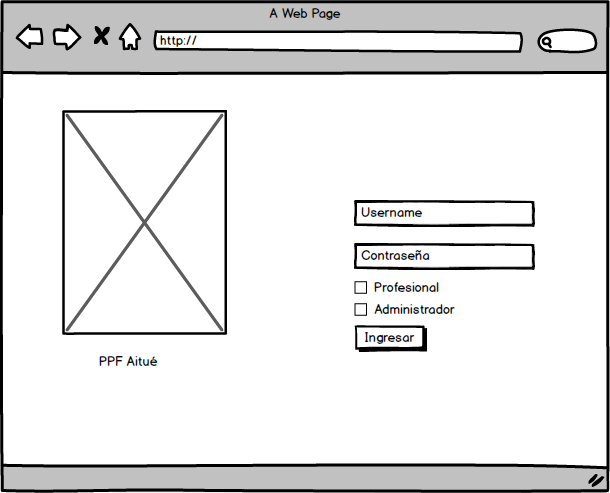
\includegraphics[scale=0.5]{imagenes/login.png}
	\end{center}
	\caption{Interfaz de inicio de la herramienta.}
\end{figure}

\clearpage
\newpage

La figura \ref{intadm} muestra la interfaz inicial luego de ingresar con la cuenta de administrador de nuestra herramienta la cual incluye una imagen representativa del PPF Aitué, el ícono con la opción de crear un nuevo usuario, modificar un nuevo usuario, ingresar al sistema y finalmente la opción de eliminar un usuario del sistema.\\


\begin{figure}[h]
	\label{intadm}
	\begin{center}
		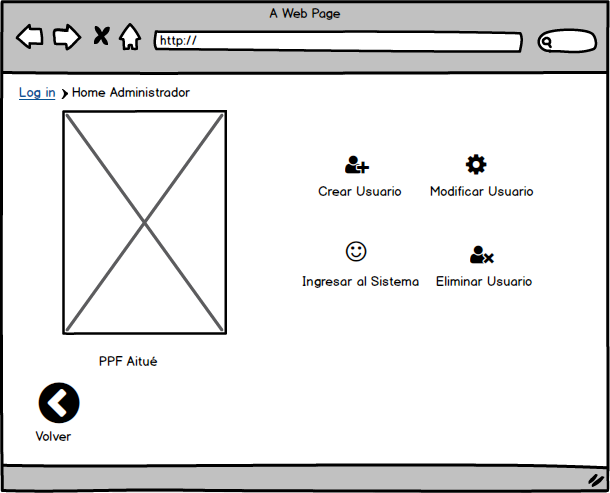
\includegraphics[scale=0.5]{imagenes/intadm.png}
	\end{center}
	\caption{Interfaz que muestra el inicio luego de ingresar como administrador.}
\end{figure}

\clearpage
\newpage

La figura \ref{newuser} muestra la interfaz luego que el administrador seleccione la opción crear usuario. Esta interfaz cuenta con un formulario que se compone de:
\begin{itemize}
	\item Nombre de usuario
	\item Contraseña
	\item Repetir contraseña
	\item Rut
	\item Mail
	\item Tipo de usuario (Psicologo o Asistente Social)
\end{itemize}

Además de una imagen representativa y en la parte inferior  los botones "Crear Usuario" y "Volver"\\

\begin{figure}[htb]
	\label{newuser}
	\begin{center}
		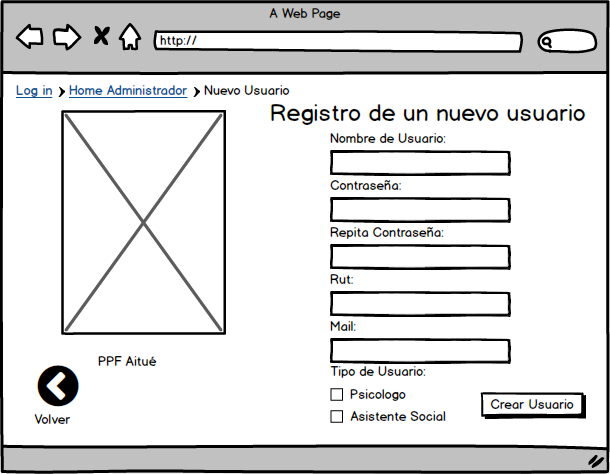
\includegraphics[scale=0.5]{imagenes/newuser.png}
	\end{center}
	\caption{Interfaz que muestra el formulario de ingreso de un nuevo usuario al sistema.}
\end{figure}

\clearpage
\newpage

La figura \ref{moduser1} muestra la interfaz luego que el administrador selecciona la opción modificar usuario, en esta interfaz se despliegan todos los usuarios almacenados en el sistema y en la parte inferior de esta lista, se muestra el botón "Modifiar usuario". \\


\begin{figure}[htb]
	\label{moduser1}
	\begin{center}
		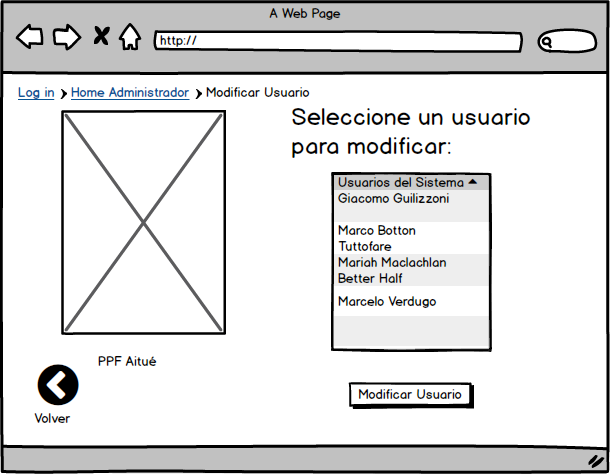
\includegraphics[scale=0.5]{imagenes/moduser1.png}
	\end{center}
	\caption{Interfaz que muestra el inicio luego de ingresar como administrador.}
\end{figure}

\clearpage
\newpage

La figura \ref{moduser} muestra la interfaz luego que el administrador seleccione la opción modificar usuario y selecciona un usuario a modificar. Esta interfaz cuenta los campos editables de:
\begin{itemize}
	\item Nombre de usuario
	\item Contraseña
	\item Mail
	\item Rut
	\item Mail
	\item Tipo de usuario (Psicologo o Asistente Social)
\end{itemize}

Además de una imagen representativa y en la parte inferior  los botones "Crear Usuario" y "Volver".\\

\begin{figure}[htb]
	\label{moduser}
	\begin{center}
		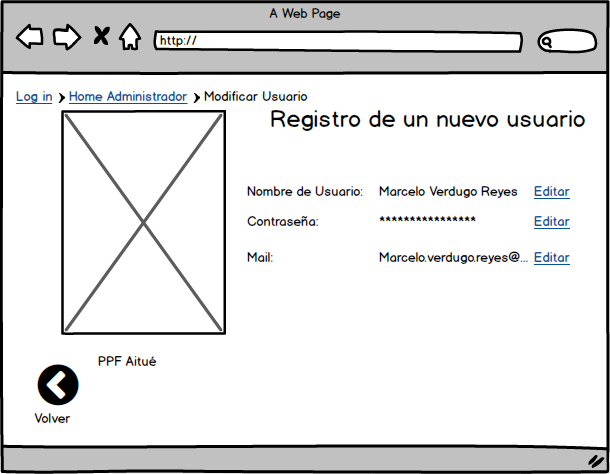
\includegraphics[scale=0.5]{imagenes/moduser.png}
	\end{center}
	\caption{Interfaz que muestra los campos editables luego de seleccionar un usuario a modificar.}
\end{figure}

\clearpage
\newpage

La figura \ref{bienvenido} muestra la interfaz luego que el administrador selecciona "Ingresar al sistema" o bien posteriormente que el profesional realiza su login.\\
En esta interfaz se muestran dos íconos representativos de la herramientas NCFAS y de la herramienta CAT-A, donde CAT-A es la herramienta del Trabajo de Título a realizar de Jean Pierre Peña. \\
Además una imagen representativa y en la parte inferior el botón "Volver".\\

\begin{figure}[htb]
	\label{bienvenido}
	\begin{center}
		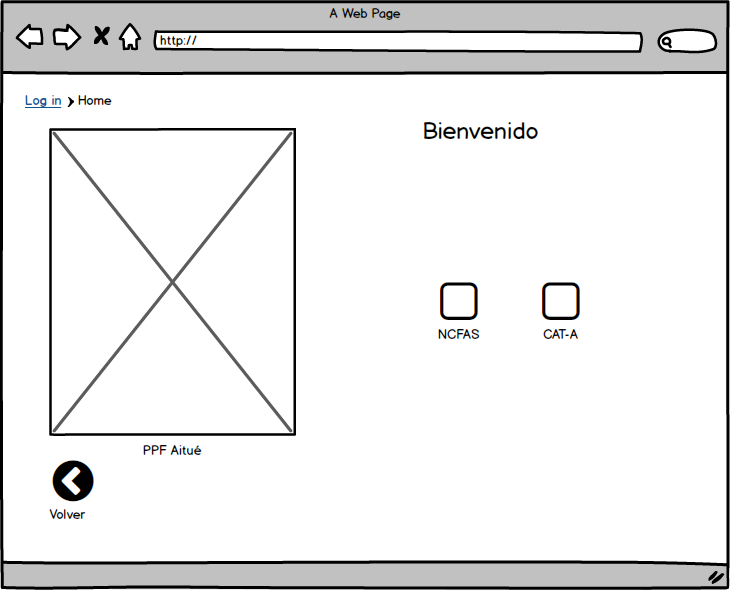
\includegraphics[scale=0.5]{imagenes/bienvenido.png}
	\end{center}
	\caption{Interfaz que muestra el inicio del sistema.}
\end{figure}

\clearpage
\newpage

La figura \ref{inicioncfas} muestra la interfaz luego que el administrador o el profesional ingresan a la herramienta NCFAS. Esta interfaz de bienvenida a la herramienta NCFAS, muetra en el costado izquierdo las posibles tareas que pueden ser realizadas por el administrador y por el profesional dentro de la herramienta NCFAS.\\

Además de una imagen representativa y de los botones "Crear Usuario" y "Volver".\\

\begin{figure}[htb]
	\label{inicioncfas}
	\begin{center}
		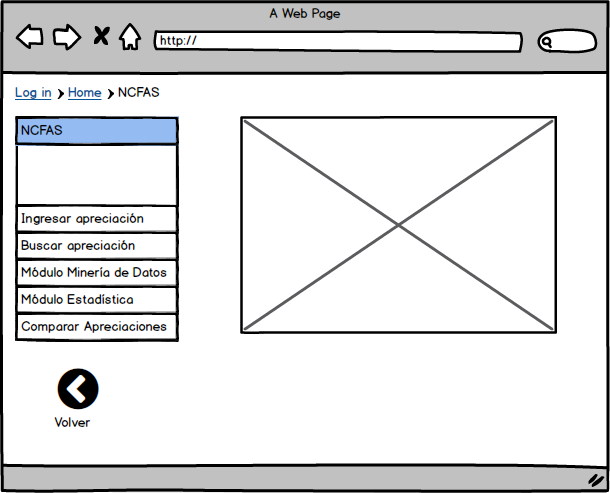
\includegraphics[scale=0.5]{imagenes/inicioncfas.png}
	\end{center}
	\caption{Interfaz que muestra el inicio luego de ingresar a la herramienta NCFAS.}
\end{figure}

\clearpage
\newpage

La figura \ref{ncfasguardados} muestra las apreciaciones guardadas en el sistema las cuales al ser seleccionadas por el administrador o por el profesional, estas pueden ser modificadas, comparadas, o bien encontrar información útil utilizando en ellas, técnicas de minería de datos o de estadística descriptiva.\\

\begin{figure}[htb]
	\label{ncfasguardados}
	\begin{center}
		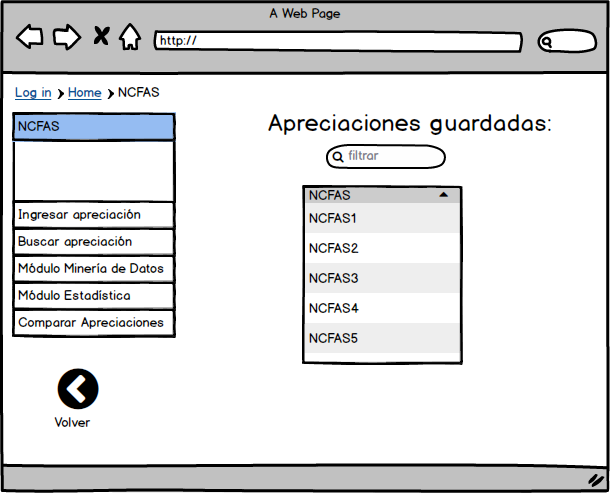
\includegraphics[scale=0.5]{imagenes/ncfasguardados.png}
	\end{center}
	\caption{Interfaz que muestra el inicio luego de ingresar a la herramienta NCFAS.}
\end{figure}

\clearpage
\newpage

La figura \ref{dimncfas} muestra las distintas dimensiones que componen la herramienta NCFAS. 
Además de las diferentes opciones que puede realizar el profesional o el administrador en el costado izquierdo, junto con el botón volver en la parte inferior izquierda.\\

\begin{figure}[htb]
	\label{dimncfas}
	\begin{center}
		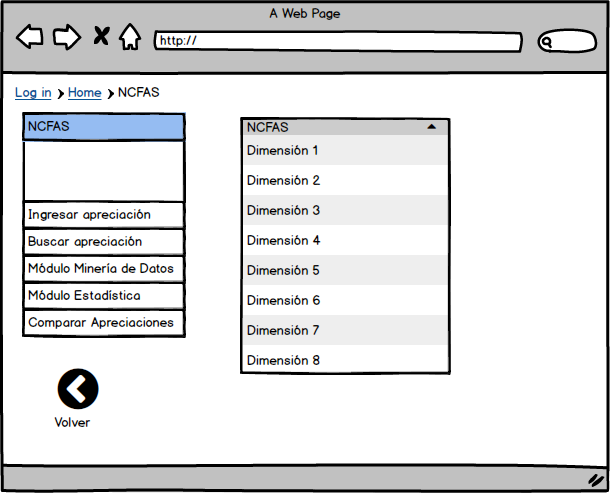
\includegraphics[scale=0.5]{imagenes/dimncfas.png}
	\end{center}
	\caption{Interfaz que muestra el inicio luego de ingresar a la herramienta NCFAS.}
\end{figure}

\clearpage
\newpage

La figura \ref{itmncfas2} muestra los distintos ítems que componen dimensiones de la herramienta NCFAS. 
Además de las diferentes opciones que puede realizar el profesional o el administrador en el costado izquierdo, junto con el botón volver en la parte inferior izquierda.\\

\begin{figure}[htb]
	\label{itmncfas2}
	\begin{center}
		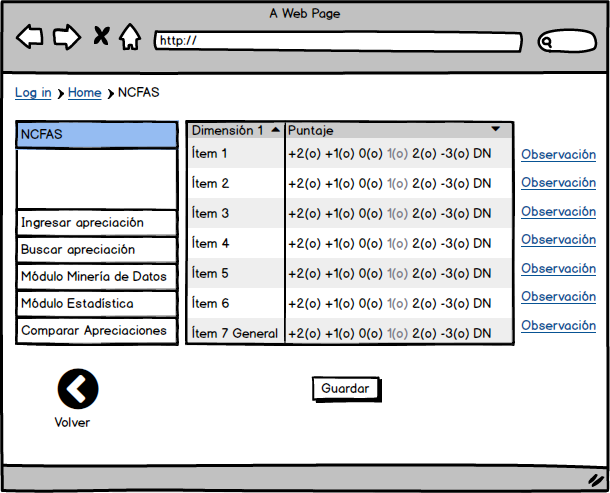
\includegraphics[scale=0.5]{imagenes/itmncfas.png}
	\end{center}
	\caption{Interfaz que muestra el inicio luego de ingresar a la herramienta NCFAS.}
\end{figure}

\clearpage
\newpage

\section{Diseño lógico} \label{disenolog}



\subsubsection{Esquemas de navegación}

\clearpage
\newpage

\subsection{Diagrama de clases}

\clearpage
\newpage

\subsection{Caso de uso reales}

En la siguiente sección se detallara la experiencia que tendrá el usuario con el sistema, mostrando cada funcionalidad. En donde los números indica donde el usuario puede interactuar con el sistema y la letra indica la interfaz a la cual se hace referencia.\\

\begin{figure}[h!]
	\label{inicioadm2}
	\begin{center}
		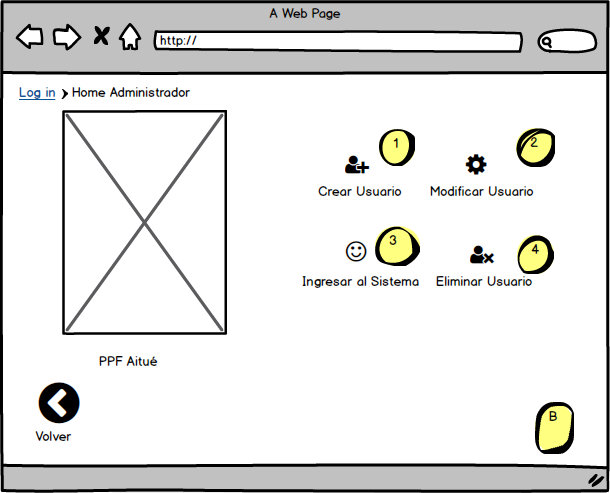
\includegraphics[scale=0.3]{imagenes/inicioadm2.png}
	\end{center}
	\caption{Interfaz que muestra el inicio luego de ingresar a la herramienta NCFAS.}
\end{figure}

\begin{figure}[h!]
	\label{formuser}
	\begin{center}
		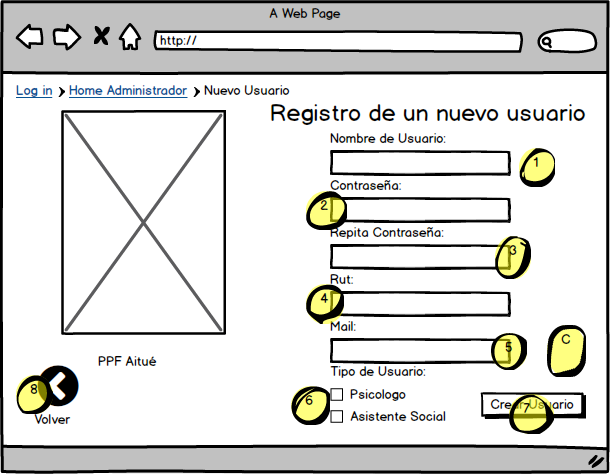
\includegraphics[scale=0.3]{imagenes/formuser.png}
	\end{center}
	\caption{Interfaz que muestra el formulario para crear un usuario.}
\end{figure}

\begin{figure}[h!]
	\label{newuseralt}
	\begin{center}
		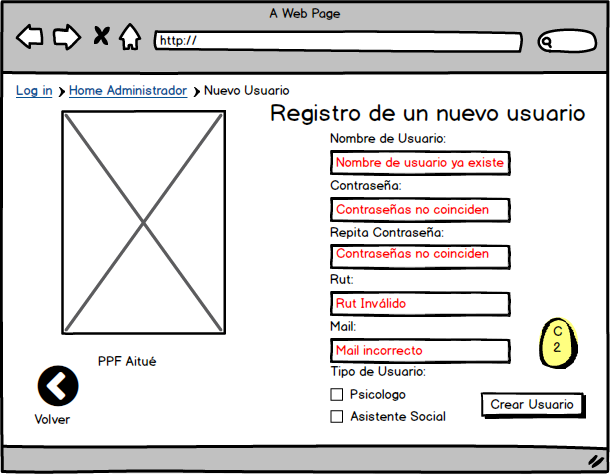
\includegraphics[scale=0.3]{imagenes/newuseralt.png}
	\end{center}
	\caption{Interfaz que muestra el formulario para crear un usuario.}
\end{figure}

\begin{table}
	\centering
	\begin{tabular}{|p{3cm}|p{3cm}|p{2.3cm} |p{3cm}|}
		\hline \textbf{Caso de Uso} & Crear Usuario & \textbf{ID} & CDU1 \\ 
		\hline \textbf{Actores} & Administrador & \textbf{Tipo} & Primario \\ 
		\hline \textbf{Pre-condición} & - & \textbf{Descripción} & Permite crear un usuario\\
		\hline \textbf{Ref. Cruzadas} & RF1 & \textbf{Resumen} & El administrador crea los usuarios asignando un respectivo nombre, e-mail, contraseña y perfil.\\ 
		\hline
	\end{tabular}  
	
	\begin{tabular}{|p{6cm}|p{6cm}|}
		
		\multicolumn{2}{|c|}{\textbf{Curso normal de eventos}} \\
		\hline \textbf{Actor} & \textbf{Sistema} \\ 
		\hline 1. Este caso de uso comienza cuando el administrador debe crear un usuario para el sistema y presiona (1B). & 2.El sistema solicita al administrador el nombre de usuario (1C), e-mail (2C), contraseña(3C) que se confirme la contraseña (4C)y que seleccione el nuevo usuario (Psicólogo o Asistente social)(5C)  \\ 
		3. El administrador ingresa lo solicitado y presiona el botón "Crear Usuario" (7C) & 4. El sistema valida lo ingresado por el administrador y crea el nuevo usuario. \\
		& 5. El sistema guarda el nuevo usuario y permite al administrador crear un nuevo usuario o bien ingresar al sistema. \\
		\hline
		\multicolumn{2}{|c|}{\textbf{Curso alternativo de eventos}} \\
		\hline
		\multicolumn{2}{|p{12cm}|}{4. El sistema valida los datos ingresados por el administrador pero estos no son válidos y vuelve al paso 3 y muestra los errores (C2).} \\
		\hline
	\end{tabular}
	\caption{Tabla del caso de uso expandido de Crear Usuario}
	\label{tabcdu1.1}
\end{table}

\clearpage


\begin{figure}[h!]
	\label{moduser2}
	\begin{center}
		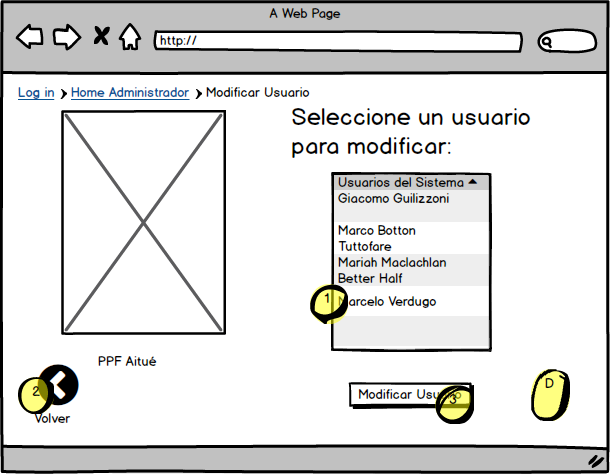
\includegraphics[scale=0.3]{imagenes/moduser2.png}
	\end{center}
	\caption{Interfaz que muestra los usuarios del sistema que se pueden modificar.}
\end{figure}

\begin{figure}[h!]
	\label{moduser3}
	\begin{center}
		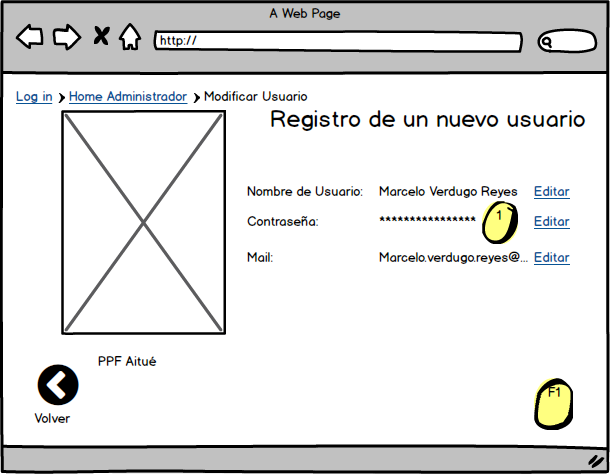
\includegraphics[scale=0.3]{imagenes/moduser3.png}
	\end{center}
	\caption{Interfaz que muestra los campos modificables del usuario.}
\end{figure}

\begin{figure}[h!]
	\label{moduser4}
	\begin{center}
		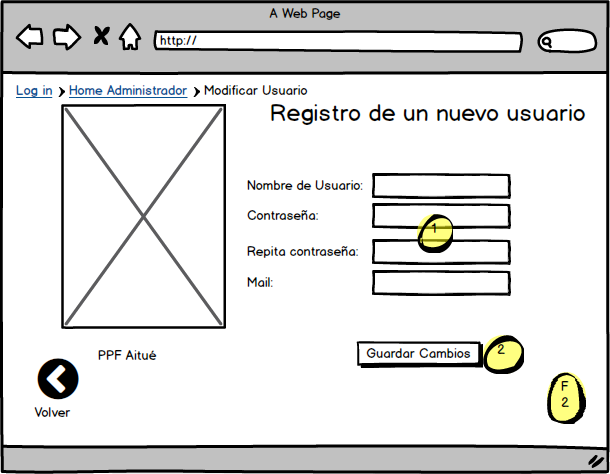
\includegraphics[scale=0.3]{imagenes/moduser4.png}
	\end{center}
	\caption{Interfaz que muestra los campos modificables del usuario.}
\end{figure}

\begin{figure}[h!]
	\label{moduser5}
	\begin{center}
		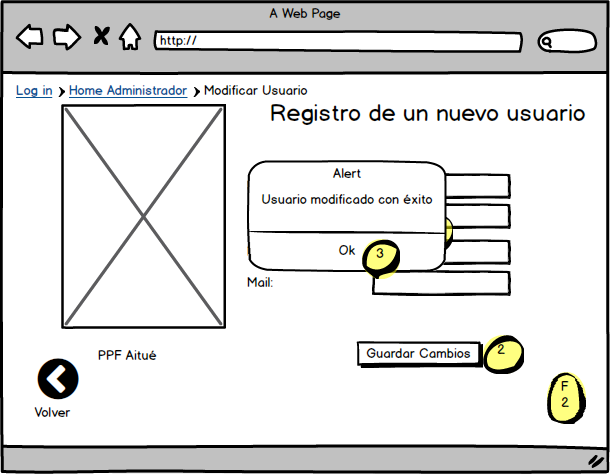
\includegraphics[scale=0.3]{imagenes/moduser5.png}
	\end{center}
	\caption{Interfaz que muestra los campos modificables del usuario.}
\end{figure}

\begin{figure}[h!]
	\label{moduser6}
	\begin{center}
		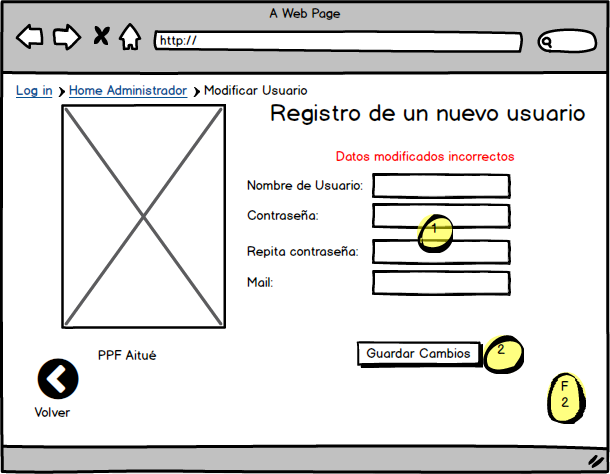
\includegraphics[scale=0.3]{imagenes/moduser6.png}
	\end{center}
	\caption{Interfaz que muestra los campos modificables del usuario.}
\end{figure}

\begin{table}
	\centering
	\begin{tabular}{|p{3cm}|p{3cm}|p{2cm} |p{3cm}|}
		\hline \textbf{Caso de Uso} & Modificar Usuario & \textbf{ID} & CDU2 \\ 
		\hline \textbf{Actores} & Administrador & \textbf{Tipo} & Opcional \\ 
		\hline \textbf{Pre-condición} & Crear un usuario & \textbf{Descripción} & Permite modificar un usuario creado anteriormente \\
		\hline \textbf{Ref. Cruzadas} & RF1 & \textbf{Resumen} & El administrador modifica un usuario creado anteriormente.\\ 
		\hline
	\end{tabular}  
	
	\begin{tabular}{|p{6cm}|p{6cm}|}
		
		\multicolumn{2}{|c|}{\textbf{Curso normal de eventos}} \\
		\hline \textbf{Actor} & \textbf{Sistema} \\ 
		\hline 1. Este caso de uso comienza cuando el administrador desea modificar un usuario creado anteriormente, seleccionando la opción modificar usuario (2B) \ref{inicioadm2}. & 2. El sistema muestra los usuarios guardados (D) \ref{moduser2}. \\ 
		3. El administrador selecciona al usuario que desea modificar(1D) \ref{moduser2} . & 4. El sistema muestra las opciones a modificar del usuario (F1) \ref{moduser3}.\\
		5. El administrador selecciona los campos a modificar (1F1) \ref{moduser2}. & 6. El sistema cambia y se adapta para recibir text imput (F2) \ref{moduser4} \\
		7. El administrador guarda las modificaciones (2F2) \ref{moduser4}. & 8. El sistema valida las modificaciones y guarda nuevamente el usuario modificado y muestra el alert (F2) \ref{moduser5} \\
		\hline
		\multicolumn{2}{|c|}{\textbf{Curso alternativo de eventos}} \\
		\hline
		\multicolumn{2}{|p{12cm}|}{7. El sistema valida los datos ingresados por el administrador pero estos no son válidos y vuelve al paso 5 \ref{moduser6}. } \\
		\hline
	\end{tabular}
	\caption{Tabla del caso de uso expandido de Modificar Usuario}
	\label{tabcdu22}
\end{table}

\clearpage

\begin{figure}[h!]
	\label{elimuser2}
	\begin{center}
		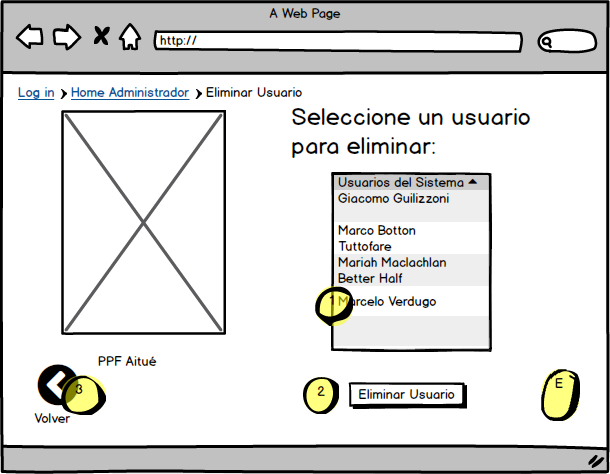
\includegraphics[scale=0.3]{imagenes/elimuser2.png}
	\end{center}
	\caption{Interfaz que muestra los campos modificables del usuario.}
\end{figure}

\begin{figure}[h!]
	\label{elimuser4}
	\begin{center}
		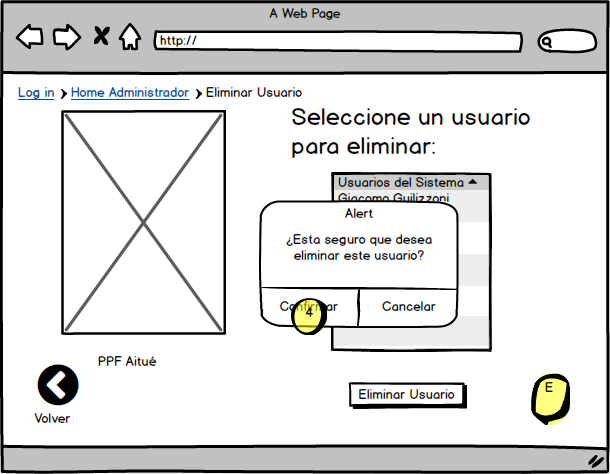
\includegraphics[scale=0.3]{imagenes/elimuser4.png}
	\end{center}
	\caption{Interfaz que muestra los campos modificables del usuario.}
\end{figure}

\clearpage

\begin{figure}[h!]
	\label{elimuser5}
	\begin{center}
		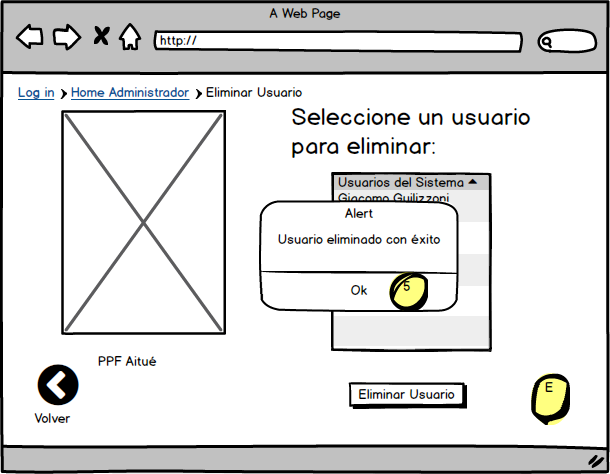
\includegraphics[scale=0.3]{imagenes/elimuser5.png}
	\end{center}
	\caption{Interfaz que muestra los campos modificables del usuario.}
\end{figure}

\begin{table}
	\centering
	\begin{tabular}{|p{3cm}|p{3cm}|p{2cm} |p{3cm}|}
		\hline \textbf{Caso de Uso} & Eliminar Usuario & \textbf{ID} & CDU3 \\ 
		\hline \textbf{Actores} & Administrador & \textbf{Tipo} & Opcional \\ 
		\hline \textbf{Pre-condición} & Crear un usuario & \textbf{Descripción} & Permite eliminar un usuario creado anteriormente \\
		\hline \textbf{Ref. Cruzadas} & RF1 & \textbf{Resumen} & El administrador elimina un usuario creado anteriormente.\\ 
		\hline
	\end{tabular}  
	\begin{tabular}{|p{6cm}|p{6cm}|}
		\multicolumn{2}{|c|}{\textbf{Curso normal de eventos}} \\
		\hline \textbf{Actor} & \textbf{Sistema} \\ 
		\hline 1. Este caso de uso comienza cuando el administrador desea eliminar un usuario creado anteriormente, seleccionando la opción eliminar usuario.(4B) \ref{inicioadm2} & 2. El sistema muestra los usuarios guardados (E) \ref{elimuser2} \\ 
		3. El administrador selecciona al usuario que desea eliminar.(1E) \ref{elimuser2} & \\
		4. El usuario presiona el botón "Eliminar Usuario" (2E) \ref{elimuser2} & 5. El sistema envía una alerta para que el administrador confirme que realmente desea eliminar el usuario seleccionado. \ref{elimuser4} \\
		6. El administrador confirma la eliminación.(4E) \ref{elimuser4} & 7. El sistema elimina al usuario y muestra una alerta (5E) \ref{elimuser5}. \\
		\hline
		\multicolumn{2}{|c|}{\textbf{Curso alternativo de eventos}} \\
		\hline
		\multicolumn{2}{|p{12cm}|}{5. El administrador cancela la eliminación del usuario y vuelve al paso 3. } \\
		\hline
	\end{tabular}
	\caption{Tabla del caso de uso expandido de Eliminar Usuario}
	\label{tabcdu33}
\end{table}

\clearpage

\begin{figure}[h!]
	\label{ncfas3}
	\begin{center}
		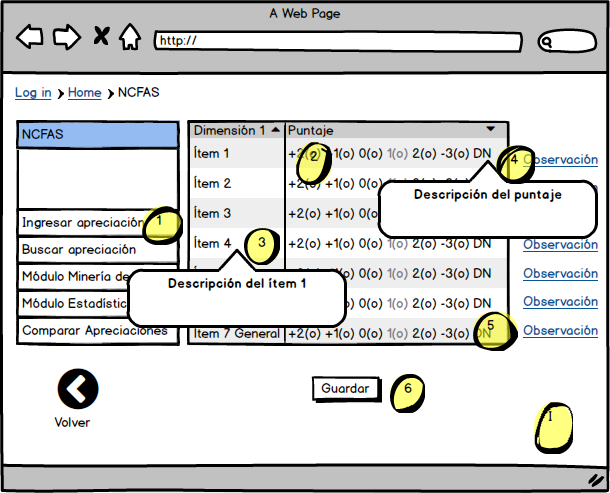
\includegraphics[scale=0.3]{imagenes/ncfas3.png}
	\end{center}
	\caption{Interfaz que muestra los campos modificables del usuario.}
\end{figure}

\begin{figure}[h!]
	\label{ncfas4}
	\begin{center}
		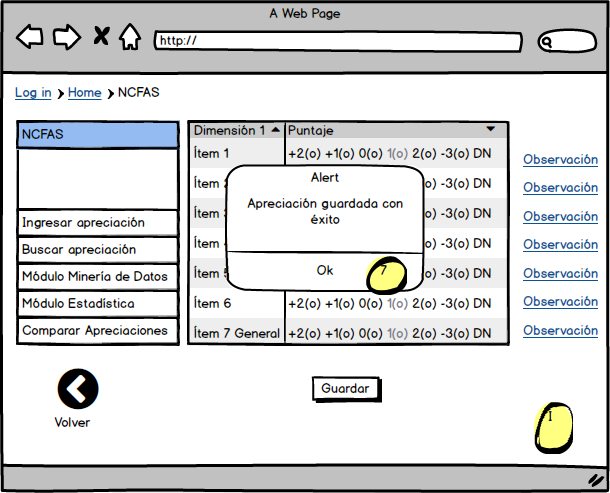
\includegraphics[scale=0.3]{imagenes/ncfas4.png}
	\end{center}
	\caption{Interfaz que muestra los campos modificables del usuario.}
\end{figure}


\begin{table}[h!]
	\centering
	\begin{tabular}{|p{2cm}|p{3cm}|p{2cm}|p{4cm}|}
		\hline \textbf{Caso de Uso} & Ingresar NCFAS & \textbf{ID} & CDU4 \\ 
		\hline \textbf{Actores} & Profesional a cargo- Administrador & \textbf{Tipo} & Primario \\ 
		\hline \textbf{Pre-condición} & - & \textbf{Descripción} & Permite ingresar una apreciación familiar mediante la herramienta NCFAS Digital \\
		\hline \textbf{Ref. Cruzadas} & RF2-RF3-RNF11 & \textbf{Resumen} & EL profesional a cargo o el administrador, luego de recopilar información necesaria de la familia, ordena y califica la información por medio de la herramienta NCFAS.\\ 
		\hline
	\end{tabular}  
	\begin{tabular}{|p{6cm}|p{6cm}|}
		
		\multicolumn{2}{|c|}{\textbf{Curso normal de eventos}} \\
		\hline \textbf{Actor} & \textbf{Sistema} \\ 
		\hline 1. Este caso de uso comienza cuando el profesional a cargo desea ingresa una nueva apreciación familiar presionando "Ingresar apreciación" (1I) \ref{ncfas3}. & 2. El sistema despliega la herramienta NCFAS Digital que se observa en (I) \ref{ncfas3}.  \\ 
		3. El profesional a cargo califica cada ítem, donde además puede ver los descriptores asociados a cada ítem (3I) y a cada puntaje asociado (4I) \ref{ncfas3}.&  \\
		4. El profesional guarda todo su progreso (6I) \ref{ncfas3}. & 5. El sistema guarda y almacena la apreciación completa y envía un alert al usuario informando que se guardó con éxito. (7C) \ref{ncfas4} \\
		\hline
		\multicolumn{2}{|c|}{\textbf{Curso alternativo de eventos}} \\
		\hline
		\multicolumn{2}{|p{12cm}|}{-} \\
		\hline
	\end{tabular}
	\caption{Tabla del caso de uso expandido de NCFAS Digital}
	\label{tabcdu44}
\end{table}

\clearpage

\begin{figure}[h!]
	\label{generainfo}
	\begin{center}
		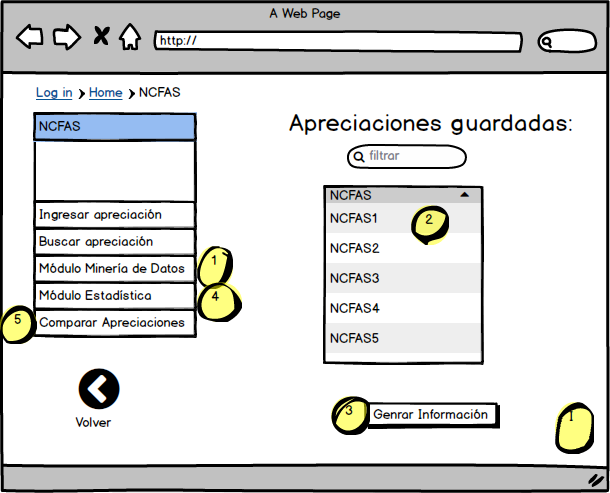
\includegraphics[scale=0.3]{imagenes/generainfo.png}
	\end{center}
	\caption{Interfaz para generar información útil a partir de las NCFAS.}
\end{figure}

\begin{figure}[h!]
	\label{estadistic}
	\begin{center}
		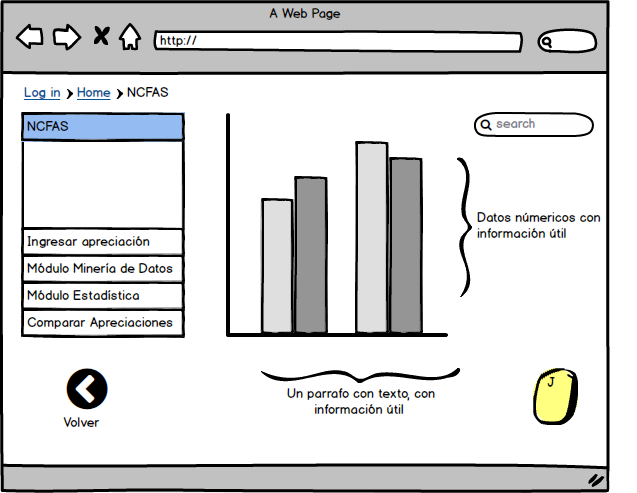
\includegraphics[scale=0.3]{imagenes/estadistic.png}
	\end{center}
	\caption{Interfaz que muestra la información utilizando técnicas de estadística descriptiva.}
\end{figure}

\begin{table}
	\centering
	\begin{tabular}{|p{6cm} |p{6cm}|}
		\hline \textbf{Caso de Uso} & Visualizar Información Estadística Descriptiva \\ 
		\hline \textbf{ID} & CDU6 \\ 
		\hline \textbf{Actores} & Profesional a cargo \\ 
		\hline \textbf{Tipo} & Opcional \\ 
		\hline \textbf{Pre-condición} & Existan apreciaciones guardadas \\ 
		\hline \textbf{Descripción} & Permite que el profesional a cargo visualice información con técnicas de Estadística Descriptiva \\
		\hline \textbf{Ref. Cruzadas} & RF4 - RF6 \\ 
		\hline
		\multicolumn{2}{|c|}{\textbf{Resumen}} \\
		\hline
		\multicolumn{2}{|p{12cm}|}{El profesional a cargo podrá visualizar la información , mediante técnicas de estadística descriptiva.} \\
		\hline 
	\end{tabular}  
	\begin{tabular}{|p{6cm}|p{6cm}|}
		\multicolumn{2}{|c|}{\textbf{Curso normal de eventos}} \\
		\hline \textbf{Actor} & \textbf{Sistema} \\ 
		\hline 1. Este caso de uso comienza cuando el profesional a cargo desea visualizar información mediante el módulo de estadística descriptiva presionando (1I) \ref{generainfo}. & 2.El sistema despliega las NCFAS guardadas para que el profesional seleccione una para generar la información.  \\ 
		3. El profesional a cargo selecciona una NCFAS (2I) \ref{generainfo}. & 4.El sistema despliega la información.(J) \ref{estadistic}  \\ 
		\hline
		\multicolumn{2}{|c|}{\textbf{Curso alternativo de eventos}} \\
		\hline
		\multicolumn{2}{|p{12cm}|}{ - } \\
		\hline
	\end{tabular}
	\caption{Tabla del caso de uso expandido de Visualizar Información Módulo Estadística Descriptiva}
	\label{tabcdu66}

\end{table}
\clearpage


\begin{figure}[h!]
	\label{min}
	\begin{center}
		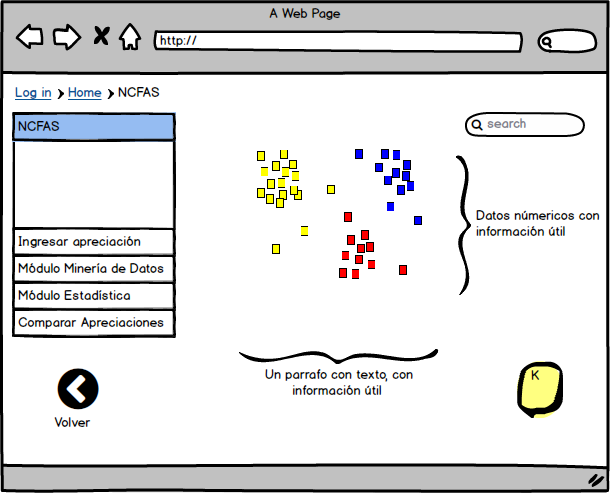
\includegraphics[scale=0.4]{imagenes/min.png}
	\end{center}
	\caption{Interfaz que muestra la información.}
\end{figure}

\begin{table}
	\centering
	\begin{tabular}{|p{6cm} |p{6cm}|}
		\hline \textbf{Caso de Uso} & Visualizar Información \\ 
		\hline \textbf{ID} & CDU7 \\ 
		\hline \textbf{Actores} & Profesional a cargo \\ 
		\hline \textbf{Tipo} & Opcional \\ 
		\hline \textbf{Pre-condición} & - \\ 
		\hline \textbf{Descripción} & Permite que el profesional a cargo visualice información con técnicas de Minería de Datos \\
		\hline \textbf{Ref. Cruzadas} & RF4 - RF6 \\ 
		\hline
		\multicolumn{2}{|c|}{\textbf{Resumen}} \\
		\hline
		\multicolumn{2}{|p{12cm}|}{El profesional a cargo podrá visualizar información mediante técnicas de minería de datos.} \\
		\hline 
	\end{tabular}  
	\begin{tabular}{|p{6cm}|p{6cm}|}
		\multicolumn{2}{|c|}{\textbf{Curso normal de eventos}} \\
		\hline \textbf{Actor} & \textbf{Sistema} \\ 
		\hline 1. Este caso de uso comienza cuando el profesional a cargo desea visualizar información mediante el módulo de minería de datos, presionando (4I) \ref{generainfo}. & 2.El sistema despliega las NCFAS guardadas para que el profesional seleccione una para generar la información.  \\ 
	El profesional a cargo selecciona una NCFAS (2I) \ref{generainfo}. & 4.El sistema despliega la información.(J) \ref{min}. \\
		\hline
		\multicolumn{2}{|c|}{\textbf{Curso alternativo de eventos}} \\
		\hline
		\multicolumn{2}{|p{12cm}|}{ - } \\
		\hline
	\end{tabular}
	\caption{Tabla del caso de uso expandido de Visualizar Información Módulo Minería de Datos}
	\label{tabcdu77}
\end{table}
\clearpage


\begin{figure}[h!]
	\label{compara}
	\begin{center}
		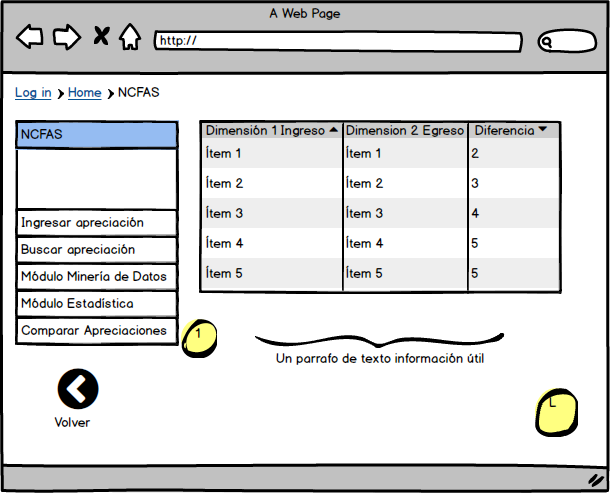
\includegraphics[scale=0.3]{imagenes/compara.png}
	\end{center}
	\caption{Interfaz que muestra la NCFAS de ingreso comparada con la NCFAS de egreso.}
\end{figure}

\begin{table}
	\centering
	\begin{tabular}{|p{6cm} |p{6cm}|}
		\hline \textbf{Caso de Uso} & Comparar NCFAS Digitales \\ 
		\hline \textbf{ID} & CDU9 \\ 
		\hline \textbf{Actores} & Profesional a cargo \\ 
		\hline \textbf{Tipo} & Opcional \\ 
		\hline \textbf{Pre-condición} & EL sistema debe tener NCFAS Digitales almacenados \\ 
		\hline \textbf{Descripción} & Permite comparar dos NCFAS(Ingreso v/s egreso) \\
		\hline \textbf{Ref. Cruzadas} & RF5 \\ 
		\hline
		\multicolumn{2}{|c|}{\textbf{Resumen}} \\
		\hline
		\multicolumn{2}{|p{12cm}|}{El profesional a cargo podrá comparar NCFAS Digitales dentro del sistema.} \\
		
	\end{tabular}  
	\begin{tabular}{|p{6cm}|p{6cm}|}
		\multicolumn{2}{|c|}{\textbf{Curso normal de eventos}} \\
		\hline \textbf{Actor} & \textbf{Sistema} \\ 
		\hline 1. Este caso de uso comienza cuando el profesional a cargo desea comparar apreciaciones familiares, presionando (5I) \ref{generainfo} & 2.El sistema despliega las NCFAS que puede seleccionar para comparar (Las que tengan una apreciación de ingreso y egreso).  \\ 
		3. El profesional a cargo selecciona las NCFAS que desea comparar, presionando (2I) \ref{generainfo}.& 4. El sistema despliega información acerca de los ítems que más variaron entre el NCFAS de ingreso v/s el NCFAS de egreso.(L) \ref{compara} \\
		\hline
		\multicolumn{2}{|c|}{\textbf{Curso alternativo de eventos}} \\
		\hline
		\multicolumn{2}{|p{12cm}|}{ - } \\
		\hline
	\end{tabular}
	\caption{Tabla del caso de uso expandido de Comparar NCFAS Digitales}
	\label{tabcdu99}
\end{table}

\clearpage

\section{Diseño de datos}  \label{disenodat}

En esta sección se detalla la creación de los archivos necesarios para poder almacenar los datos de las apreciaciones familiares y, posteriormente llevar a cabo las técnicas de minería de datos y estadística descriptiva. 

\subsection{Archivo ARFF}

En la herramienta NCFAS existen 8 dimensiones en dónde cada una de estas se compone de diferentes ítems, a su vez, cada ítem puede ser calificado con distintos valores, los que son:

\begin{itemize}
	\item NA (No aplica): Cuando no es necesario evaluar este ítem
	\item +2: El cual indica, una Clara Fortaleza 
	\item +1: El cual indica, una leve Fortaleza
	\item 0: El cual indica, una Linea de Base Adecuado
	\item -1: El cual indica, una Problema Leve
	\item -2: El cual indica, una clara Problema Moderado
	\item -3: El cual indica, una clara Problema Serio
	\item DN (Desconocido): Cuando se desconoce que valor otorgar a este ítem
\end{itemize}

Un ejemplo de una dimensión con sus respectivos ítem es la Figura \ref{escalaejem}.\\

\begin{figure}[h!]
	\label{escalaejem}
	\begin{center}
		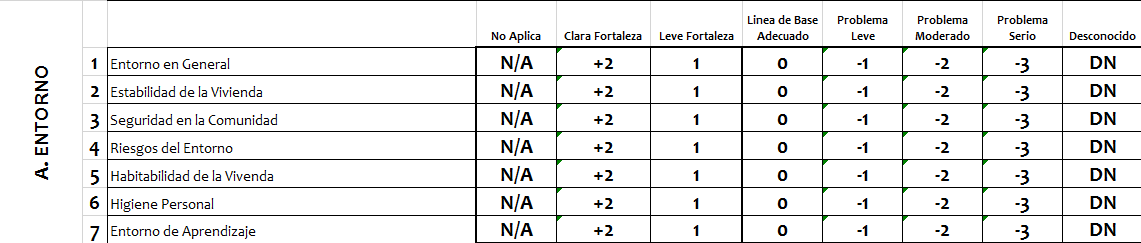
\includegraphics[scale=0.4]{imagenes/escalaejem.png}
	\end{center}
	\caption{Figura ejemplo de un ítem de la herramienta NCFAS con su respectiva escala de valores.}
\end{figure}



La forma en la que será representado esto se realizará con un archivo ARFF un archivo ARFF (Attribute-Relation File Format) es un archivo de texto ASCII que describe una lista de instancias que comparten un conjunto de atributos.\\
Un archivo ARFF se compone de dos secciones. La primera de la cabecera de la información seguida por los datos. La cabecera contiene los nombres de las relaciones, una lista de atributos y sus tipos.

El nombre del archivo ARFF a utilizar se compondrá del Nombre de la Familia seguido de un número identificador como muestra la siguiente figura \ref{archivo}. 

\begin{figure}[h!]
	\label{archivo}
	\begin{center}
		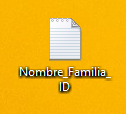
\includegraphics[scale=0.3]{imagenes/archivo.png}
		\caption{Figura que representa el archivo generado al realizar una apreciación familiar.}
	\end{center}
\end{figure}

Los datos que contendrá nuestro archivo ARFF con el fin de representar lo mostrado en la figura \ref{escalaejem} será de la siguiente manera:

\begin{figure}[h!]
	\label{cabecera}
	\begin{center}
		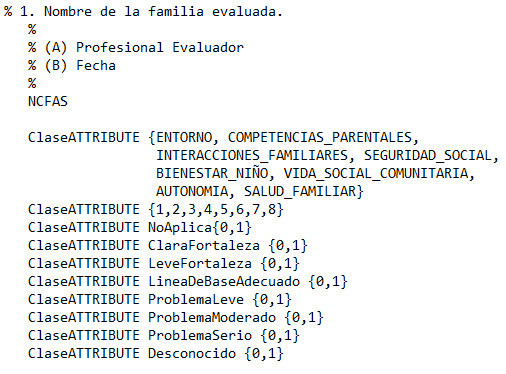
\includegraphics[scale=0.4]{imagenes/cabecera.png}
		\caption{Figura que representa la forma en que los datos serán representados en nuestro sistema.}
	\end{center}
\end{figure}



En esta figura encontramos el detalle de los diferentes datos que se guardarán luego de realizar una apreciación familiar por parte del profesional a cargo, el cual contiene información acerca de la familia evaluada, nombre del profesional a cargo y fecha.\\ Seguido del "ClaseATTRIBUTE" de la dimensión posteriormente "ClaseATTRIBUTE" del número del ítem de esta dimensión. Seguido de los valores que puede tomar la escala que van desde N/A hasta Desconocido. En dónde solo uno de este conjunto tendrá asignado el valor "1".\\

Un ejemplo de lo descrito anteriormente sería el siguiente vector de entrada: 

\begin{figure}[h!]
	\label{data}
	\begin{center}
		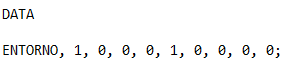
\includegraphics[scale=0.4]{imagenes/data.png}
		\caption{Figura que representa los datos de una apreciación familia.}
	\end{center}
\end{figure}

En este caso en particular el primer dato que encontramos en este vector corresponde a la dimensión "ENTORNO", posteriormente se tiene un número que va desde 1 hasta 8, el cual representa 1 de los 8 ítems de la "Dimensión Entorno" seguido del vector representativo de la escala de evaluación. En este caso particular el el valor marcado corresponde a "Leve Fortaleza".\\

Los elementos como se aprecia en la imagen, están separados entre ellos por "comas" y al final de cada uno de ellos existirá un "punto y coma" para diferenciar que viene otro conjunto de datos. \\

\clearpage
\newpage


 \section{Diseño de pruebas}
 Debe definir cuidadosamente el objetivo y como realizará las pruebas de cada parte de su desarrollo:  Pruebas de requerimientos, Pruebas de análisis,  Pruebas de diseño, Pruebas de unidad, Pruebas de integración. Pruebas de sistema. Pruebas de aceptación del usuario, entre otras.\\
 
 \clearpage
 \newpage


\section{Conclución}  \label{conclusiones}
Incluya análisis crítico sobre  pertinencia del problema, solución propuesta, proyecciones
y estado de avance. Extensión máxima sugerida 2 páginas.\\
\clearpage
\newpage
